\chapter{Determining What Makes an Effective Developer Recommendation}
\label{chap-peer}

This chapter presents studies evaluating two different techniques for recommending developer behaviors, namely \textit{peer interactions} and the \tele. To explore what makes effective recommendations to software engineers, we analyze in-person tool recommendations between users completing tasks and introduce a baseline automated approach in a simple bot for making recommendations to software engineers to gain insight into what makes a compelling developer recommendation and motivate the need for a new technique. Additional details and study materials for these experiments can be found in Appendix A.

\section{Peer Interactions}

\textit{Peer interactions} are defined as the process of software engineers learning about development tools and practices from colleagues in-person during normal work activities~\cite{Murphy-Hill2011PeerInteraction}. Murphy-Hill and colleagues examined different modes of development tool discovery among software engineering, including peer interactions and other technical approaches such as random tool encounters in development environments, tutorials, descriptions or mentions online or in publications, discussion threads, social media sites such as Twitter and RSS Feeds, and comments and discussion in online forums, and found that peer interactions are the most effective way developers discover new software engineering tools~\cite{Murphy-Hill2011PeerInteraction}. Furthermore, software engineering literature shows peer interactions are useful for supporting additional developer behaviors such as increasing adoption of security tools to help developers build more secure systems by detecting security vulnerabilities~\cite{Xiao2014Security}, increasing collaborative development practices~\cite{Kalliamvakou15OSSCollaborative}, and improving how developers understand and share knowledge about their code~\cite{Maalej2014CodeComprehension}. Little is known about the nature of peer interactions, and to explore what makes these user-to-user recommendations effective I performed a user study to observe and analyze tool recommendations between peers.

\subsection{Study Rationale}

To increase awareness of useful tools and features designed to help users in software, recommender systems can automatically suggest beneficial tools to users. However, despite the large number of automated recommender systems, prior work suggests user-to-user peer interactions are the most effective method for tool discovery~\cite{Murphy-Hill2011PeerInteraction}. There is limited research exploring why face-to-face recommendations between peers are effective increasing tool adoption, and to better understand why users prefer recommendations from colleagues this work administers a user study to analyze different characteristics of the recommendations. The characteristics we analyzed are motivated by existing literature in psychology and persuasion theory, as well as prior software engineering research examining peer interactions. The results of this work provide insights into why in-person tool recommendations between peers are effective and implications for improving automated recommender systems.

\subsubsection{Research Question}

To examine the influence of peer interactions on recommendations between software users, this work sought to answer the following research question:

\begin{itemize}
    \item[\textbf{RQ1}] What characteristics of peer interactions make recommendations effective?
\end{itemize}

To answer this question, we investigated the effectiveness of peer interactions by conducting a user study to observe tool recommendations between 13 pairs of participants completing data analysis tasks. We analyzed the peer interactions by recognizing tool recommendations between partners, observing how tools were suggested based on different recommendation characteristics, and detecting how often suggestions were adopted or ignored by participants. The main contribution of this work is a study to characterize how software users make tool recommendations to peers.

\subsection{Peer Interaction Characteristics}

To analyze the effectiveness of peer interactions, we explored six characteristics of recommendations between partners in our user study: politeness, persuasiveness, receptiveness, time pressure, tool observability, and peer interaction type. These characteristics are motivated from research exploring the delivery of messages to humans in psychology and software engineering. Here, I provide examples for each characteristic from prior work and present the criteria used to identify instances of each attribute in tool recommendations between participants in this study:

% We used literature from other fields to compile a list of criteria for politeness, persuasiveness, and receptiveness defined with examples from this evaluation in Tables~\ref{tab:politeDef}-\ref{tab:receptiveDef}. For each characteristic, we analyzed comments made in the dialogue between participants during peer interactions to observe these criteria. 

\textit{Politeness.} Prior work suggests politeness is a key factor for making effective suggestions to humans. For example, Whitworth suggests many existing recommendation techniques, such as pop-up ads and the Microsoft Clippy recommender system, are ineffective and unpopular among users because it was impolite~\cite{WhitworthPolite}. In software engineering, researchers have explored incorporating politeness into sentiment analysis tools to observe programmers~\cite{danescuniculescumizil2013computational}, and show this concept can encourage developers to fix issues faster and increase work satisfaction in agile development teams~\cite{Ortu15WouldYouMind}.
To measure politeness in peer interactions, we used Leech's six maxims for politeness: Tact, Generosity, Approbation, Modesty, Agreement, and Sympathy~\cite{LeechPragmatics}. The definition of these criteria and examples from the experiment can be found in Table~\ref{tab:politeDef}.

\textit{Persuasiveness.} Social psychology posits persuasion theory, or the study of the communication of messages to affect the attitudes and behavior of humans~\cite{Gardikiotis15Persuasion}. Research suggests persuasiveness is crucial for making effective recommendations. For instance, O'Keefe argues ``human decision-making is shaped by persuasive communication''~\citep[p.~31]{okeefe2002persuasion}. Fogg also suggests persuasiveness is also necessary to convince users to adopt desired behaviors through software~\cite{Fogg2009Persuasive}. For example, Faridi and colleagues propose integrating persuasion into the software development lifecycle to help reduce problems developers face while building software products~\cite{faridi2012human}. Shen et al. introduce a generic model for developing persuasive messages including three features: Content, Structure, and Style~\cite{ShenMessageFeatures}. We used these criteria defined in Table~\ref{tab:persuasiveDef} to measure the persuasiveness of recommendations between participants in this study.

\textit{Receptiveness.} Psychology literature shows receptiveness plays an important role in the adoption of recommendations. For example, Feng argues receptiveness is necessary for humans to receive advice from others during problematic situations~\cite{feng2006receptiveness}. Research also shows receptiveness is beneficial for adopting multicultural experiences and accepting ideas from foreign cultures~\cite{leung2010multicultural}. Prior work in software engineering has also explored using openness, one of the five personality domains~\cite{digman1990personality}, to observe the practices of developers~\cite{smith2016beliefs}. Fogg argues receptiveness is vital for creating persuasive technology to persuade users to adopt beneficial behaviors online~\cite{Fogg2009Persuasive}. To define receptiveness, he posits two criteria which are used in this study to measure this characteristic within peer interactions between participants: Demonstrate Desire and Familiarity. Definitions of these criteria and examples derived from our user study are presented in Table~\ref{tab:receptiveDef}.

\textit{Time Pressure.} Research from various disciplines shows time pressure impacts recommendations to humans. In behavioral economics, Kocher and colleagues suggest the allotted time to make decisions impacts the quality of choices because ``time \textit{is} money''~\cite{kocher2006time}. In marketing, studies show time constraints damage decision-making by stifling creativity and reducing exploratory thinking~\cite{AndrewsTimePressure}. Furthermore, software engineering research asserts time pressure from deadlines negatively impacts development practices~\cite{CostelloDeadline84} and prevents peer interactions~\cite{Murphy-Hill2015HowDoUsers}. To measure time pressure in recommendations between participants in this study, we analyzed sessions to search for discussions about time between partners. Time limits were not strictly enforced in the study, but sessions lasted one hour and we recommended spending 7–8 minutes on each question. If we determined a statement regarding time was made during a peer interaction, then the recommendation was categorized as being under time pressure. An example of the criteria used to measure time pressure is available in Table~\ref{tab:timeDef}.

\textit{Tool Observability.} Observability refers to whether or not systems consist of interfaces visible to users, which studies suggest influences the adoption of tools and behaviors. For instance, research shows visual attention, or the perceptual analysis of humans on various sensory features such as size, shape, and color, impacts the brands of products consumers purchase~\cite{pieters1999visualattention}. Furthermore, Nielsen submits ``Visibility of system status'' as a usability heuristic for designing usable user interfaces~\cite{nielsen1993usability}. Murphy-Hill and colleagues suggest systems should have noticeable causes and effects to improve tool discoverability for software engineers~\cite{Murphy-Hill2015HowDoUsers}. 
To analyze this, we examined the observability of tools recommended between participants in the study. To evaluate the impact of the perception of tools on the outcome of peer interactions, we analyzed tools suggested between participants in our study to categorize them as Observable or Non-observable. Table~\ref{tab:toolDef} presents the definitions of these criteria and examples from the study.

\textit{Peer Interaction Type.} Murphy-Hill and colleagues found peer interactions are the most effective mode of tool discovery among software engineers. They introduce two types of peer interactions, \textit{peer observations} and \textit{peer recommendations}~\cite{Murphy-Hill2011PeerInteraction}, that differ in how suggestions are instigated between colleagues. Peer observation refers to when a developer views a colleague using an unfamiliar tool, while peer recommendations occur when colleagues notice coworkers completing tasks inefficiently and recommend a tool. Peer interactions were categorized as Peer Observations or Peer Recommendations based on the analysis of recommendations between participants.

\begin{table}[p!]
\centering
\begin{center}
\caption{Definition and examples of the politeness peer interaction characteristic}
    \begin{tabular}{ |l|l|p{10cm}| }
		\hline
	\multicolumn{3}{ |c| }{\textbf{Politeness Criteria}} \\
	\hline
	\multirow{3}{*}{Tact} 
	 & Definition & Minimize cost and maximize benefit to peer \\
	 & Polite & \textit{``We can do all of it together, just sort by level.''} (S9) \\
	 & Impolite & \textit{``We can do a histogram...which is always sort of a pain in the butt to do in Excel.''} (L14) \\ \hline
	\multirow{3}{*}{Generosity} 
	 & Definition & Minimize benefit and maximize cost to self \\
	 & Polite & \textit{``CONCATENATE you can do. I can do this for
you, very easily.''} {S10} \\
	 & Impolite & \textit{``Maybe you should write a python script for this.''} {L6} \\ \hline
	\multirow{3}{*}{Approbation} 
	 & Definition & Minimize dispraise and maximize praise of peer \\
	 & Polite & \textit{``I'm not as good at the Excel stuff as you are.''} (L5) \\
	 & Impolite & \textit{``This[partner's suggestion] is useless.''} (S14) \\ \hline
	\multirow{3}{*}{Modesty} 
	 & Definition & Minimize praise and maximize dispraise of self \\
	 & Polite & \textit{``From whatever limited knowledge of data analysis I have, I think you need to create a linear regression model...''} (S14) \\
	 & Impolite & \textit{``I'm very good at Paint.''} (S10) \\ \hline
	\multirow{3}{*}{Agreement} 
	 & Definition & Minimize disagreement and maximize agreement between peers \\
	 & Polite & \textit{``Do you want to use Python?''} (S8) \\
	 & Impolite & \textit{``No, no, no...Don't you want it comma separated? That's what I'm doing.''} (S14) \\ \hline
	\multirow{3}{*}{Sympathy} 
	 & Definition & Minimize antipathy and maximize sympathy between peers\\
	 & Polite & \textit{``We can try JMP...'' [``I haven't done anything in JMP.''] ``Neither have I!''} (L14) \\
	 & Impolite & \textit{``It doesn't matter how you do it.''} (L16) \\ \hline
\end{tabular}
\label{tab:politeDef}
\end{center}
\end{table}

\begin{table}[p!]
\centering
\begin{center}
\caption{Definition and examples of the persuasiveness peer interaction characteristic}
    \begin{tabular}{ |l|l|p{10cm}| }
		\hline
	\multicolumn{3}{ |c| }{\textbf{Persuasiveness Criteria}} \\
	\hline
	\multirow{3}{*}{Content} 
	 & Definition & Recommender provides credible sources to verify use of the tool\\
	 & Persuasive & \textit{``Go here, go to Data. Highlight that...Data, Sort, and it lets you pick two.''} (L8) \\
	 & Unpersuasive & \textit{``Let's try to text filter, right?''} (S5) \\ \hline
	\multirow{3}{*}{Structure} 
	 & Definition & Messages are organized by climax-anticlimax order of arguments and conclusion explicitness \\
	 & Persuasive & \textit{``I know that SUMIF is a type of function that allows you to combine the capabilities of SUM over a range with a condition that needs to be met.''} (S3)\\
	 & Unpersuasive & \textit{``There's a thing on Excel where you can do that, where you can say if it is this value, include, if it is not, exclude...Yeah, IF.''} (S11) \\ \hline
	\multirow{3}{*}{Style} 
	 & Definition & Messages should avoid hedging, hesitating, questioning intonations, and powerless language \\
	 & Persuasive & \textit{``Control-Shift-End''} (S1) \\
	 & Unpersuasive & \textit{``I guess we're going to have to use some math calculations here, or a pivot table.''} (L9) \\ \hline
\end{tabular}
\label{tab:persuasiveDef}
\end{center}
\end{table}

\begin{table}[p!]
\centering
\begin{center}
\caption{Definition and examples of the receptiveness peer interaction characteristic}
    \begin{tabular}{ |l|l|p{9cm}| }
		\hline
	\multicolumn{3}{ |c| }{\textbf{Receptiveness Criteria}} \\
	\hline
	\multirow{3}{*}{Demonstrate Desire} 
	 & Definition & User showed interest in discovering, using, or learning more information about the suggested tool \\
	 & Receptive & \textit{``That was cool, how [the column] just populated.''} (S4) \\
	 & Unreceptive & \textit{[``So you want to use R for it?''] ``No, no, no...''} (S14) \\ \hline
	\multirow{3}{*}{Familiarity} 
	 & Definition & User explicitly expresses familiarity with the environment \\
	 & Receptive & \textit{``Control shift...how do I select it completely?''} (S2) \\
	 & Unreceptive & \textit{``I've never done anything in JMP.''} (L10) \\ \hline
\end{tabular}
\label{tab:receptiveDef}
\end{center}
\end{table}

\begin{table}[p!]
\centering
\begin{center}
\caption{Definition and examples of the time pressure peer interaction characteristic}
    \begin{tabular}{ |l|l|p{9cm}| }
		\hline
	\multicolumn{3}{ |c| }{\textbf{Time Pressure Criteria}} \\
	\hline
	\multirow{3}{*}{Time Pressure} 
	 & Definition & Participant makes statement regarding time after a recommendation \\
	 & Yes & ``\textit{Yeah, that would work if we had time.}'' (L5) \\
	 & No & No comments about time \\ \hline
\end{tabular}
\label{tab:timeDef}
\end{center}
\end{table}


\begin{table*}[ht]
\centering
\begin{center}
\caption{Definition and examples of the tool observability peer interaction characteristic}
    \begin{tabular}{ |l|l|p{9cm}| }
	\hline
	\multicolumn{3}{ |c| }{\textbf{Tool Observability Criteria}} \\
	\hline
	\multirow{3}{*}{Observability} 
	 & Definition & The ability to view the recommended tool through a graphical user interface \\
	 & Observable & ``\textit{Let's deploy a histogram}...[In Menu] \textit{Insert, Recommended Charts...}'' (S7) \\
	 & Non-Observable &  ``\textit{Control-Shift-End}'' (S1) \\ \hline
\end{tabular}
\label{tab:toolDef}
\end{center}
\end{table*}



\subsection{Methodology}

To observe these characteristics in peer interactions and investigate their effectiveness as a recommendation approach, I implemented a mixed methods approach to analyze using grounded theory and statistical data analysis techniques to examine the impact of each characteristic on observed tool recommendations between peers.

\subsubsection{Data Collection}

\paragraph*{Participants}

To evaluate peer interactions, we observed pairs of participants working together to complete data analysis tasks. Participants were students from various disciplines at North Carolina State University and professional analysts from the NC State Laboratory for Analytic Sciences\footnote{\url{https://ncsu-las.org/}} (LAS). For the remainder of this section, student participants are delineated with the S- prefix and LAS participants are presented with the L- prefix. More details about the user study participants can be found in Appendix~\ref{app-peer-participants}. Overall, 13 pairs completed the study, seven pairs of students and six pairs of professional analysts.

\paragraph*{Tasks}

Participants were asked to complete data analysis tasks based on the Kaggle Titanic data science competition.\footnote{\url{https://www.kaggle.com/c/titanic}} The specific study tasks given to participants are available in Appendix~\ref{app-peer-tasks}. The dataset for the tasks consisted of two comma-separated values files, \textsc{train.csv} and \textsc{test.csv}. The training tasks required participants to analyze the \textsc{train.csv} file containing information about Titanic passengers to observe patterns and correlations in the data based on the survival of individuals. The testing task required participants to analyze the \textsc{test.csv} files, which contained a different set of passengers and no details about their survival, and use their analysis from the preliminary tasks to predict whether individuals survived the shipwreck. While we provided solutions to the final tasks, the intent of this study was not to scrutinize the correctness or efficiency of solutions but to investigate how participants recommended tools to each other to solve the problems. 

\paragraph*{Study Design}

Pairs of subjects were provided with one machine to work together to complete the tasks. The experiment machine was a Windows 10 laptop with several data analysis programs installed including Microsoft Excel 2016,\footnote{\url{https://products.office.com/en-us/excel}} JMP Pro 12,\footnote{\url{http://www.jmp.com/en_us/home.html}} MySQL Workbench 6.3,\footnote{\url{http://www.mysql.com/products/workbench/}} Python 2.7,\footnote{\url{https://www.python.org/}} PyCharm,\footnote{\url{https://www.jetbrains.com/pycharm/}} R (command line and GUI),\footnote{\url{https://www.r-project.org/}} and RStudio.\footnote{\url{https://www.rstudio.com/}} Participants were permitted to request and download additional free and publicly available software applications to analyze the data, however they were prohibited from using the Internet to complete the tasks to prevent looking up information about the problem and requiring participants to only rely on their own knowledge of tools to complete the tasks. Screen and voice recordings of participants completing the task were captured to further observe and analyze characteristics of tool recommendations between pairs. 

Additionally, participants weer asked to provide qualitative data after sessions to further analyze peer interactions observed during studies. To debrief participants, we emailed a survey (students) and conducted a semi-structured interview (LAS) to ask subjects about tool recommendations that occurred during the study. The guiding questions for the semi-structured interview are available in Appendix~\ref{app-peer-interview}. Additionally, participants were asked to complete a demographic survey (Appendix~\ref{app-peer-survey}) to collect information about our study population.


\subsubsection{Determining the effectiveness of peer interactions} 

Two independent researchers viewed the recordings from each study session to note instances of tool recommendations, categorize the recommendation based on our peer interaction characteristics, and determine the outcome of the recommendation. We iteratively define coding criteria for identifying and characterizing instances of peer interactions. Each recording was analyzed to determine:
\begin{itemize}[topsep=0pt,itemsep=-1ex,partopsep=1ex,parsep=1ex]
    \item when a tool recommendation took place
    \item if the recommendation was effective
    \item if the recommendation was polite, persuasive, receptive, under time pressure, or made about observable tools
\end{itemize}

More details about the specific information collected for each peer interaction observed in this evaluation are provided in Appendix~\ref{app-peer-data}. Below, I describe our process for identifying peer interactions, determining the existence of each characteristic, and evaluating the effectiveness of recommendations.

\paragraph*{Identifying peer interactions}

To identify peer interactions between participants, I developed a model to define tool recommendations based on the GOMS (Goals, Operators, Methods, and Selection rules) model in Human-Computer Interaction~\cite{diaper2003handbook}. This model, shown in Figure~\ref{fig:peer-model}, outlines how we recognized peer interactions between two participants. Each node indicates a step required to denote an instance of a peer interaction. To describe this model, I use terms for developers in a pair programming environment where the user actively operating the keyboard and mouse is the driver and the peer observing is the navigator~\cite{Cockburn01Pair}. 

During \textit{task analysis}, both users consider the problem and develop a strategy to complete the task. \textit{Task execution} refers to users discovering a mismatch between their task solution strategies. For peer observations, the navigator observes the driver completing the task using an unfamiliar tool. Peer recommendations occurs when the navigator notices deficiencies in the driver's approach and desires to suggest a better strategy. Finally, in the \textit{dialogue} step a tool is recommended between the users. We transcribed recommendations to analyze the dialogue and determine the type of recommendation. For example, during peer observations the navigator may inquire about the driver's unknown tool. For peer recommendations, the navigator would suggest a tool to complete the task more efficiently or the may driver seek help. Two researchers independently analyzed the recordings of participant pairs completing the tasks and used this model to determine instances of peer interactions between partners.

\paragraph*{Characterizing peer interactions}

After identifying tool recommendations between participants, the two coders analyzed each peer interaction instance to determine if each of our peer interaction characteristics, politeness, persuasiveness, receptiveness, time pressure, tool observability, and interaction type, play a role in the effectiveness of recommendations. We used a valence scale to calculate scores for categorizing recommendations based on politeness (\textit{polite, neutral, impolite}), persuasiveness (\textit{persuasive, unpersuasive}), and receptiveness (\textit{receptive, neutral, unreceptive}) according to our criteria defined for each trait (see Tables~\ref{tab:politeDef}-\ref{tab:receptiveDef}):

\begin{itemize}[topsep=0pt,itemsep=-1ex,partopsep=1ex,parsep=1ex]
    \item[\textbf{+1}] Participant obeyed a specific characteristic criteria
    \item[\textbf{0}] Participant neither obeyed nor violated a specific characteristic criteria
    \item[\textbf{-1}] Participant violated a specific characteristic criteria
\end{itemize}

This scale was used by the coders to classify peer interactions individually, then we came together to discuss and resolve disagreements. A positive result indicates the existence of a characteristic, while a negative sum signifies the characteristic was not present. The definitions of the scoring criteria implemented to identify these characteristics, which we arrived at iteratively, is available in Appendix~\ref{app-peer-scoring}. We used Cohen's Kappa to calculate the inter-rater agreement for politeness ($\kappa$ = 0.50), persuasiveness ($\kappa$ = 0.28), and 
receptiveness ($\kappa$ = 0.51). A binary scale was implemented to measure time pressure (\textit{time pressure, no time pressure}) and tool observability (\textit{observable, non-observable}) based on the criteria in Tables~\ref{tab:timeDef} and \ref{tab:toolDef} as well as the type of peer interaction. 

\paragraph*{Determining effectiveness}

After identifying instances of software tool recommendations between participants, the two coders analyzed each interaction to categorize them as \textit{effective}, \textit{ineffective}, and \textit{unknown}. Effective recommendations indicate the recommendee, or participant receiving the tool suggestion, used a tool after it was suggested by their partner for a majority of the relevant tasks. For ineffective recommendations, the recommendee mostly ignored the tool suggested by their partner when given the opportunity to apply it. Finally, since the study consisted of two participants working together on the same computer, there were cases of unknown recommendations where there was no opportunity for the recommendee to use the suggested tool for the rest of the study session. To resolve disagreements between the two coders, we watched the recording clip of the peer interaction instance in question together, each explained our reasoning behind our individual coding, discussed the rationale for each code, and came to an agreement.

\begin{figure}
    \centering
    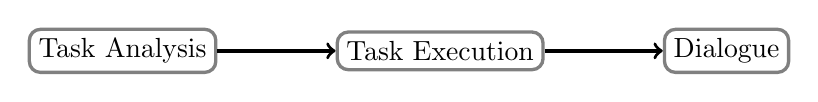
\begin{tikzpicture}
        \node[right] at (0, 0) (task)[rectangle, rounded corners, text centered, draw=gray, very thick] {Task Analysis};
        \draw [very thick, ->] (task.east) -- ++(1.5cm, 0) 
            node[right] (exec)[rectangle, rounded corners, text centered, draw=gray] {Task Execution};
        \draw [very thick, ->] (exec.east) -- ++(1.5cm, 0)
            node[right] (dial)[rectangle, rounded corners, text centered, draw=gray] {Dialogue};
        \end{tikzpicture}
    \caption{Model to identify peer interactions between participants}
    \label{fig:peer-model}
\end{figure}



\subsection{Results}

We identified a total of 142 peer interactions from our user study, categorizing 71 as effective, 35 as ineffective, and 36 as unknown. Study pairs averaged approximately 11 tools recommended between participants within each session. To quantitatively analyze the data collected from the experiment, the Mann-Whitney-Wilcoxon (W) test was used to evaluate ordinal data (\textit{politeness}, \textit{persuasiveness}, and \textit{receptiveness}) and Pearson’s chi-squared ($\chi^2$) test was used to evaluate categorical data (\textit{time pressure} and \textit{tool observability}). All statistical tests were calculated with an alpha level of $\alpha=.05$ and odds ratios (OR) were used to measure effect size.

\begin{figure}
\centering
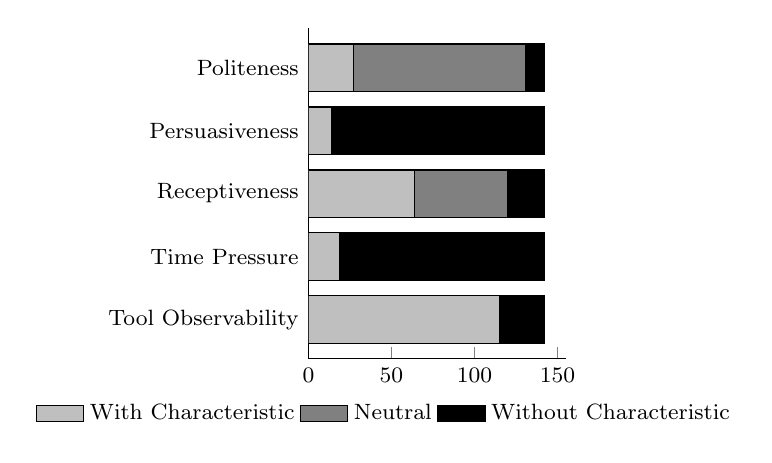
\begin{tikzpicture}
\begin{axis}[
    xbar stacked,
    legend style={
    legend columns=3,
        at={(xticklabel cs:0.3)},
        anchor=north,
        draw=none
    },
    ytick=data,
    axis y line*=none,
    axis x line*=bottom,
    tick label style={font=\footnotesize},
    legend style={font=\footnotesize},
    label style={font=\footnotesize},
    xtick={0,50,100,150},
    width=.4\textwidth,
    bar width=6mm,
    xlabel= Number of Recommendations,
    yticklabels={Tool Observability, Time Pressure, Receptiveness, Persuasiveness, Politeness},
    xmin=0,
    xmax=155,
    area legend,
    y=8mm,
    enlarge y limits={abs=0.625},
]
% With
\addplot[fill=lightgray] coordinates
{(115,0) (19,1) (64,2) (14,3) (27,4)};
% Neutral
\addplot[fill=gray] coordinates
{(0,0) (0,1) (56,2) (0,3) (104,4)};
% Without
\addplot[fill=black] coordinates
{(27,0) (123,1) (22,2) (128,3) (11,4)};
\legend{With Characteristic, Neutral, Without Characteristic}
\end{axis}  
\end{tikzpicture}
\caption{Peer Interaction Characteristic Results}
\label{fig:peer-chars}
\end{figure}

\subsubsection{Characteristics}

Each of the peer interactions observed between participants were categorized based on the peer interaction characteristics and their overall effectiveness. Figure~\ref{fig:peer-chars} displays the number of recommendations that meet each of the characteristics for peer interactions we observed, and Table~\ref{tab:peer-results} displays the effectiveness of recommendations based on the peer interaction 
characteristics.

\begin{table*}[!htbp]
\centering
\caption{Peer Interaction Effectiveness Results}
\resizebox{0.85\textwidth}{!}{%
\begin{tabular}{|l|lll|lll|lll|}
\hline
  \multirow{2}{*}{}  &  \multicolumn{3}{c|}{Effective} & \multicolumn{3}{c|}{Ineffective} & \multicolumn{3}{c|}{Unknown}  \\
\cline{2-10}
 & \textit{n} & & \% & \textit{n} & & \% & \textit{n} & & \% \\
\hline
\multicolumn{8}{|l}{\textit{Politeness}} &  & \\
\hline
Polite & 14 & \posbar{.52} & 52\% & 5 & \posbar{.19} & 19\% & 8 & \posbar{.30} & 30\% \\
Neutral & 52 & \neutralbar{.5} & 50\% & 27 & \neutralbar{.26} & 26\% & 25 & \neutralbar{.24} & 24\% \\
Impolite & 5 & \negbar{.45} & 45\% & 3 & \negbar{.27} & 27\% & 3 & \negbar{.27} & 27\%\\
\hline
\multicolumn{8}{|l}{\textit{Persuasiveness}} &  & \\
\hline
Persuasive & 5 & \posbar{.36} & 36\% & 4 & \posbar{.29} & 29\% & 5 & \posbar{.36} & 36\% \\
Unpersuasive & 66 & \negbar{.52} & 52\% & 31 & \negbar{.24} & 24\% & 31 & \negbar{.24} & 24\%\\
\hline
\multicolumn{8}{|l}{\textit{Receptiveness*}} &  & \\
\hline
Receptive & 39 & \posbar{.61} & 61\% & 9 & \posbar{.14} & 14\% & 16 & \posbar{.25} & 25\% \\
Neutral & 27 & \neutralbar{.48} & 48\% & 14 & \neutralbar{.25} & 25\% & 15 & \neutralbar{.27} & 27\% \\
Unreceptive & 5 & \negbar{.23} & 23\% & 12 & \negbar{.55} & 55\% & 5 & \negbar{.23} & 23\%\\
\hline
\multicolumn{8}{|l}{\textit{Time Pressure}} &  & \\
\hline
Yes & 7 & \posbar{.37} & 37\% & 7 & \posbar{.37} & 37\% & 5 & \posbar{.26} & 26\% \\
No & 64 & \negbar{.52} & 52\% & 28 & \negbar{.23} & 23\% & 31 & \negbar{.25} & 25\%\\
\hline
\multicolumn{8}{|l}{\textit{Tool Observability}} &  & \\
\hline
Observable & 57 & \posbar{.50} & 50\% & 30 & \posbar{.26} & 26\% & 28 & \posbar{.24} & 24\% \\
Non-Observable & 14 & \negbar{.52} & 52\% & 5 & \negbar{.19} & 19\% & 8 & \negbar{.30} & 30\% \\
\hline
\multicolumn{8}{|l}{\textit{Recommendation Type}} &  & \\
\hline
Peer Observation & 16 & \posbar{.30} & 30\% & 5 & \posbar{.09} & 9\% & 32 & \posbar{.60} & 60\% \\
Peer Recommendation & 55 & \negbar{.62} & 62\% & 30 & \negbar{.34} & 34\% & 4 & \negbar{.05} & 5\%\\
\hline
\end{tabular}
}
\label{tab:peer-results}
\end{table*}

\paragraph*{Politeness}

Our analysis shows the majority of participants did not make polite recommendations according to our politeness criteria, classifying 27 tool recommendations between peers as polite, 11 as impolite, and 104 as neutral. Overall, while polite recommendations were more likely to be adopted than impolite ones ($OR = 0.6786$), politeness did not significantly impact the outcome of peer interactions (W, $p = 0.4936$).

\paragraph*{Persuasiveness}

Additionally, we discovered participants were rarely persuasive during peer interactions; there were only 14 persuasive recommendations in total while 128 were unpersuasive  according to our study criteria. While prior work suggests persuasiveness is an important characteristic for convincing users to adopt desired behaviors, this characteristic did not significantly influence the effectiveness of tool recommendations between participants (W, $p = 0.4556$, $OR = 1.4722$).

\paragraph*{Receptiveness}

We found most of the peer interactions in our study incorporated receptiveness, categorizing 64 as receptive, 56 as neutral, and 22 as unreceptive. Overall this characteristic had a high rate of effectiveness, with 61\% of receptive peer interactions leading to the adoption of the recommended tool. Furthermore, we found receptiveness significantly impacts the outcome of tool recommendations between peers (W, $p = 0.0002, OR = 0.2840$). We expand on this finding in the Summary.

\paragraph*{Time Pressure}

Only 19 peer interactions observed between participants were categorized as being under time pressure. Similar to prior work, we found tool recommendations between peers without time pressure were more effective (52\%) and more than twice as likely to be accepted by participants compared to those where time pressure was present ($OR = 2.2857$). However, this characteristic did not play a significant role in the outcome of peer interactions ($\chi^2$, $p = 0.1470$).

\paragraph*{Tool Observability}

Observable tools were far more recommended during peer interactions in our study, with 115 recommendations compared to 27 non-observable tools. However, we found non-observable tool recommendations were slightly more effective (52\%). Examples of observable tools recommended in our study include applications such as R and software features like Sort and pivot tables in Excel. Non-observable tools were primarily keyboard shortcuts. We found that the observability of tools did not significantly impact the effectiveness of recommendations ($\chi^2$, $p = 0.4928$, $OR = 2.4060$).
 
\paragraph*{Peer Interaction Type}

In our analysis, we found that peer recommendations ($n$ = 89) occurred more often than peer observations ($n$ = 53). This indicates software users are more likely to make suggestions for tools and features as opposed to observing a tool and seeking information. Although tools recommended through peer recommendations are more likely to be adopted by users than peer observations (62\%), this difference was not statistically significant ($\chi^2$, $p = 0.3163$, $OR= 0.5729$).

\subsubsection{Summary}

Our results were unable to show that politeness, persuasiveness, time pressure, observability, and interaction type influence tool recommendations between peers. However, we discovered that receptiveness was the only characteristic to significantly impact the outcome of peer interactions. Thus, we conclude no matter how polite, persuasive, time-constrained, or visible a recommendation for a system is, users will not adopt a tool unless they are receptive to using it. The receptiveness characteristic is also the most difficult to implement, since it solely depends on how recommendees receive and respond to suggestions, which recommenders cannot control. Our findings suggest peer interactions are effective because of their ability to foster user receptivity. To define receptiveness, we used criteria from prior work~\cite{Fogg2009Persuasive} that suggests users must demonstrate \textbf{\em desire} and \textbf{\em familiarity} to be receptive to recommendations. We further expound on these criteria in the Discussion.

\section{\TELE}

The \tele is a basic approach for making automated recommendations to software engineers. This technique is referred to as a telemarketer design because behaves similar to a telemarketer that ``calls'' users to deliver static messages, never deviates from the script, and lacks the social context necessary to adjust messages, customize recommendations, or respond to questions and feedback. I developed this technique to define a baseline approach for recommending useful developer behaviors to programmers, such as static analysis tool adoption. With the \tele, a system sends developers a generic message with information about a tool, provides a random example featuring a code snippet incorporating a common programming error irrelevant to the program, and provides the sample output from the tool given this vague error. To evaluate this naive design, I developed a simple bot to identify a baseline for making automated recommendations to software engineers and to better understand how developers respond to recommendations from automated systems.

\subsection{Study Rationale}

While peer interactions are the most effective method of tool discovery, Murphy-Hill and colleagues also discovered they occur infrequently in the workplace~\cite{Murphy-Hill2011PeerInteraction}. Furthermore, Turkle argues technology has become a substitute for face-to-face communications between humans~\cite{turkle2017alone}. Thus, as peer interactions are in decline, it is becoming increasingly important to develop automated systems to recommend developer behaviors. Software engineering research shows bots are useful for automating a variety of programming tasks to improve developer productivity~\cite{storey2016bots}. However, studies also show bots can also be inconvenient and frustrating during interactions with humans~\cite{Hill2015Chatbots, Stanfill86MemBasedReasoning}. To better understand the impact of bots on recommendations to developers, we evaluated the \tele baseline approach in \toolone, an automated system for making development tool recommendations to software engineers on GitHub. In this study, we examined the effectiveness of recommendations from \toolone and gathered feedback from developers who received suggestions from thus system to better understand the impact of automated recommender bots and set the groundwork for designing better solutions in future approaches.


\subsubsection{Research Questions}

In this work, we explored the effectiveness of automated recommendations from bots by using the \tele to discover:

\begin{itemize}[topsep=0pt,itemsep=-1ex,partopsep=1ex,parsep=1ex]
  \item[\textbf{RQ1}] How well do bots encourage developers to adopt useful software engineering practices?
  \item[\textbf{RQ2}] How do developers respond to receiving recommendations from bots?
\end{itemize}

In this evaluation, the goal was to initiate and then identify reactions from developers to evaluate the \tele recommendations in \toolone. The results suggest bots with limited technical knowledge and generic recommendations are ineffective for influencing programmer behavior, and responses from developers provide insight into \toolone was inadequate and implications for improving future systems. This work contributes the \tele, a simple method that provides a baseline for designing automated recommendations, \toolone, a bot that incorporates the \tele to recommend static analysis tools to developers, to motivate the need for new automated recommendation approaches.

\subsection{\toolone: Implementing the \tele} 

To evaluate the \tele, I developed \toolone to generate automated tool recommendations to developers. This bot integrates the \tele by automatically making generic recommendations and adding static analysis tools on repositories using automated pull requests on GitHub. Pull requests are the preferred method to propose changes to GitHub repositories~\cite{PullRequests}, and prior work suggests automated pull requests are useful for upgrading out-of-date dependencies~\cite{Samim2017AutoPullRequests} and fixing static analysis tool violations~\cite{C-3PR}. The initial implementation of \toolone in this evaluation naively recommends \EP, an open source Java static analysis tool,\footnote{\url{http://errorprone.info/}} to developers on GitHub (see Figure~\ref{fig:tool-recommender-bot}a). To automatically integrate \EP into projects, \toolone adds the \EP plugin to repositories that utilize the Maven automation and dependency management tool for Java applications by updating the Project Object Model (\pom) build configuration file to run the tool when the code compiles (Figure~\ref{fig:tool-recommender-bot}b). 

Figure~\ref{fig:sorry-rec} provides a closer look at the automated pull request recommendation text from this system to show how the \tele is implemented in \toolone. First, the recommendation provides generic information about the \EP Java static analysis tool (Fig.~\ref{fig:sorry-rec}.A). Then, the bot also presents a simple example of a Java coding error, using the ``\texttt{==}'' operator to evaluate string equality instead of the \texttt{String.equals()} function (Fig.~\ref{fig:sorry-rec}.B1), and provides the corresponding output from \EP based on the given \texttt{StringEquality} error\footnote{\url{http://errorprone.info/bugpattern/StringEquality}} (Fig.~\ref{fig:sorry-rec}.B2). Ineptly, this simple error may not be present in the program and is irrelevant to the code base of project. An example pull request from our system using the \tele on our repository can be found here\footnote{\url{https://github.com/CSC-326/JSPDemo/pull/2}} and is available in Appendix~\ref{app-sorry}.
% \begin{figure*}[htbp]
% \centering
\begin{figure*}[]
\centering
\subfloat[Pull request recommendation text]{\includegraphics[width=0.45\linewidth]{Chapter-3/images/botse1.png}}
\subfloat[Pull request diff updating a \pom file]{\includegraphics[width=0.5\linewidth]{Chapter-3/images/botse2.png}}
\caption{Example automated pull request from \toolone}
\label{fig:tool-recommender-bot}
\end{figure*}

\begin{figure}[h]
\centering
	\includegraphics[width=\textwidth]{Chapter-3/images/tool-recommender-bot.png}
	\caption{\TELE recommendation}
	\label{fig:sorry-rec} 
\end{figure}




\subsection{Methodology}

To observe the \tele as a baseline for automated recommendations, I designed a mixed methods study to analyze the effectiveness of \toolone recommendations and collect feedback from developers to further evaluate this simple approach and gain insight into improving future automated recommender systems.

\subsubsection{Data Collection}

\paragraph*{Projects}

To evaluate the baseline \tele approach, \toolone sent automated recommendations to developers working on real-world software applications. The projects used for the evaluation were public open source software repositories on GitHub randomly sampled from the evaluation for Repairnator~\cite{Repairnator}, an automated program repair bot.\footnote{\url{https://github.com/Spirals-Team/repairnator/blob/master/resources/data/results-buildtool.csv}} To be eligible for this experiment, projects selected for the study had to meet the following criteria:

\begin{itemize}[topsep=0pt,itemsep=-1ex,partopsep=1ex,parsep=1ex]
    \item written in Java 8 or higher,
    \item successfully validate and compile with Maven,
    \item do not already include \EP in the build configuration
\end{itemize}

Due to the fact that \EP analyzes Java code, our evaluation was limited to projects written in that programming language. To determine projects that build with Maven, we checked to ensure repositories contained a \pom file in the highest-level directory and confirmed the project could be validated and compiled before adding the tool plugin. We also verified that projects did not already utilize \EP by analyzing \pom files to make sure the \EP plugin was not present to avoid making recommendations to projects that already use the tool and target developers less likely to know about it. Overall, we identified 52 projects that met these criteria to use for this study. The list of GitHub repositories used in the evaluation of the \tele in \toolone is available in Appendix \ref{app-sorry-projects}. These selected projects that received automated pull request recommendations from our bot varied in functionality, programming language, contributions, and size. 

\subsubsection{Determining the effectiveness of \tele recommendations}

To evaluate the \tele, we categorized recommendations as \textit{effective} and \textit{ineffective} based on the status of automated pull requests from \toolone. On GitHub, developers have the option to merge pull requests and incorporate them into the repository\footnote{\url{https://docs.github.com/en/enterprise-server@2.22/github/collaborating-with-issues-and-pull-requests/merging-a-pull-request}} or close pull requests without merging them.\footnote{\url{https://docs.github.com/en/enterprise-server@2.22/github/collaborating-with-issues-and-pull-requests/closing-a-pull-request}}. Additionally, developers can also ignore pull requests by leaving them open. For our evaluation, merged automated pull requests indicated an effective recommendation because developers showed a willingness to try \EP and adopt the recommended tool into their repository by merging the changes from \toolone into their code base. For example, in the pull-based software development model, merged pull requests indicate contributions from external developers are approved to be integrated into the source code for a repository~\cite{gousios2014exploratory}. Alternatively, closed or ignored pull requests implied the recommendation was ineffective. The \tele pull request recommendations were monitored for one week to categorize the recommendations. 

To assess the baseline \tele automated recommendation approach, we calculated the rate of effectiveness was calculated by measuring the percentage of merged pull requests out of the 52 \toolone recommendations sent. Additionally, we aggregated comments from GitHub developers on pull requests to analyze how programmers reacted to receiving a \tele recommendation on their repository. In \toolone automated pull requests, our bot encouraged developers to provide feedback on recommendations by asking developers to ``Please feel free to add any comments below explaining why you did or did not find this recommendation useful''. This qualitative data was compiled and analyzed to determine how developers reacted to receiving \tele recommendations from a bot and collect feedback on this simple approach.

\subsection{Results}

The \toolone system sent 52 automated pull requests recommending \EP to developers on GitHub using the \tele. On these recommendations, we received a total of 24 comments from developers or other automated systems. To analyze the data collected, we calculated the merge rate of pull request recommendations from \toolone and examined feedback from programmers to determine effectiveness.

\begin{table}[h]
\centering
\caption{\toolone Effectiveness Results}
\begin{tabular}{ |c|c|c| } \hline
  & \textit{\textbf{n}} & \textbf{Merge Rate} \\ \hline
 Merged & 2 & 4\% \\ \hline 
 Closed & 10 & 19\% \\ \hline
 No Response & 40 & 77\%\\ \hline 
\end{tabular}
\label{tab:sorry-results}
\end{table}


\subsubsection{Recommendation Effectiveness}

Our findings show that the \tele is not effective for influencing developer behavior (see Table~\ref{tab:sorry-results}). In this evaluation, \toolone was only able to make two successful recommendations out of 52 total notifications (4\%). The remaining automated pull requests, 10 closed and 40 receiving no response from developers, resulted in an overwhelming 96\% of \toolone recommendations categorized as ineffective. Furthermore, while two recommendations from our system were merged, in one case a GitHub issue was created to report problems with the project build based on the changes by \toolone and the pull request was reverted in a later pull request to remove \EP from the project. Even though the tool was eventually removed, we still categorize this instance as an effective recommendation because the developers accepted the pull request and tried the tool before removing it.

\subsubsection{Feedback}

Overall, we observed 24 total pull request comments on 17 unique projects that received recommendations from \toolone. Of the 24 comments, six were made by automated systems on the pull requests to provide information for first-time contributors, request Contributing License Agreement (CLA) signatures, or present code coverage updates. Thus, we received 18 responses from 15 individual developers on 14 recommendations, most of which was negative feedback. Additionally, of the recommendations that received feedback from developers through pull request comments ($n = 14$), 86\% were ineffective and immediately rejected and closed by users ($n = 11$) or left open and never revisited by a developer ($n = 1$). 

While we received some positive reactions from developers on \toolone recommendations, even on those that were not merged (i.e. ``\textit{lgtm, Good Contribution}'' (P9), ``\textit{Thanks for sharing it}''(P13)), the majority of feedback was poor (i.e. ``Please stop using automated tools with a lack of understanding against random repos on github.'' (P6), ``\textit{Automated advertising is spam!}'' (P8)). Overall, the analysis of developer comments posits the main criticisms from developers were about breaking builds ($n = 8$) and messing up the \pom formatting ($n = 5$). We further investigate this feedback to provide themes describing why the \tele in \toolone was ineffective.

\subsection{Summary}

Our results suggest simple bots are ineffective for influencing the behavior of developers. Most \tele recommendations were ineffective, ignored or rejected by developers. This motivates the need for new design approaches and improvements to recommender bots to enhance recommendations and encourage developers to adopt better behaviors. Based on feedback from developers who received naive recommendations from \toolone, we discovered the main drawbacks of the \tele are a lack of \textit{\textbf{social context}} and interrupting \textit{\textbf{developer workflow}}. These concepts are explained and further outlined in the Discussion section.

\section{Discussion: \textit{Developer Recommendation Preconditions}}


Based on the results from these preliminary studies, we uncovered four concepts useful for designing automated behavioral recommendations to developers based on the efficacy of peer interactions and inadequacy of the \tele: \textbf{\em desire}, \textbf{\em familiarity}, \textbf{\em social context}, and \textbf{\em developer workflow}. At a minimum, automated recommender systems must incorporate these \textit{developer recommendation preconditions} in order to make convincing recommendations for software engineers. Below we explore each concept, providing definitions, examples from the completed evaluations, and illustrations from existing software engineering literature.

\subsection{Desire}

Demonstrating desire, or users expressing eagerness to adopt recommended tools and practices, led to effective recommendations between participants in the peer interactions user study. For example, in peer interaction observed during the study participant L12 recommended using the multi-level sorting functionality in Excel. Their partner, L11, demonstrated a desire to use this feature by responding ``\textit{Oh! Add level! Yes, awesome!}'', and the multi-level sorting tool was adopted for completing the rest of the study tasks. Meanwhile, in another session one participant recommended using R for analyzing data to complete a task, but their partner responds ``\textit{No, no, no...}'' (S14). This suggests recommending desirable tools and behaviors can increase adoption among developers, while a lack of desire can negatively impact the outcome of a recommendation. 

Software engineering research also suggests desire impacts the adoption of activities and behavior by developers. For instance, Senyard and colleagues suggest desire is important for motivating programmers to contribute to and maintain successful open source software projects~\cite{senyard2004have}. Furthermore, Murphy-Hill and colleagues found that one barrier to the adoption of useful development tools and practices is \textit{developer inertia}, which refers to when programmers are unwilling to switch from their current workflow and do \textit{not} desire to share or learn about new software engineering tools because they ``feel that they do not need to discover a new tool because existing tools will do the job''~\cite{Murphy-Hill2015HowDoUsers}. Prior work proposes using history-based recommender systems to track user behavior and recommend desirable tools based on their activity~\citep[p.~16]{Murphy-Hill2012Fluency}. To effectively recommend developer behaviors useful for completing programming tasks, recommendations must include desirable and advantageous tools and practices to encourage adoption by developers.

\subsection{Familiarity}

Another takeaway from the peer interactions user study is that users are more likely to adopt recommendations for well-known and recognizable tools and concepts. We observed comments from participants explicitly expressing familiarity and knowledge about recommended tools or their functionality. For instance, in one interaction when L8 recommended using the \texttt{COUNTIF} function in Excel, L7 was familiar with the feature and navigated to the menu to adopt the tool replying ``\textit{Yeah...here we go}''. On the other hand, we found unfamiliar tools negatively impacted recommendations. For example, when a S10 proposed using R to complete a task, their partner responded ``\textit{I don’t know R}'' (S9), and the partner's unfamiliarity with R led to an ineffective recommendation. According to our results, recommending familiar tools can increase the effectiveness of recommendations for developer behavior. This points to a need to incorporate familiar concepts to developers when recommending beneficial development tools and practices.

There are several ways familiarity can impact behavior adoption. For example, familiarity can also lead to \textit{developer inertia}, where programmers prefer familiar tools and processes over of adopting new systems. Prior work also suggests increasing employee knowledge about their workplace and environment, or \textit{work familiarity}, improves their performance~\cite{goodman1992familiarity}. In software engineering, research shows familiarity impacts the completion of tasks and coordination among distributed development teams~\cite{espinosa2002shared}, increasing code comprehension, or familiarity with code, improves development practices~\cite{ko2006exploratory}, and unfamiliarity in the Eclipse\footnote{https://www.eclipse.org/ide/} development environment led to disorientation and decreased productivity~\cite{de2006using}. To incorporate familiarity, prior work propose using history-based systems ranking commands based on similarity using collaborative filtering~\cite{Murphy-Hill2012Fluency}. Additionally, existing recommender systems posit organization-wide learning~\cite{linton2000owl} and collecting user history from networked workstations~\cite{ToolBox} to suggest tools used by colleagues in similar circumstances.

\subsection{Social Context}

The results from the \tele~study show this approach was ineffective because of its lack of social context. This refers to the standard practices and community activities necessary to participate in software engineering by interacting with developers and contributing to projects. Examples of these activities include adhering to formatting and style guidelines, participating in code review discussions, and agreeing to CLAs. The most common complaint we received from GitHub users on \toolone recommendations related to social context was that this system did not follow project style guidelines and disconfigured the whitespace of \pom files when automatically adding the \EP plugin (see Figure~\ref{fig:tool-recommender-bot}b). For example, developers replied ``\textit{The automated tool you use messed up the pom.xml formatting to an extent that I could not see it}'' (P5) and ``\textit{This change removes quite a lot if important things from the POM file}'' (P7), even though \toolone only added the \EP plugin and nothing was removed from configuration files. This suggests our bot's inability to conform to the social context surrounding software development discouraged developers from adopting recommendations.

Social aspects of computing play a major role in making recommendations to developers. For example, prior work argues software engineering is a social activity~\cite{ahmadi2008survey}, peer interactions between colleagues are the most effective mode of tool discovery~\cite{Murphy-Hill2011PeerInteraction}, social media has changed the way developers learn about and share new information~\cite{begel2010social, singer2014twitter}, and social factors influence the adoption of security development tools~\cite{Xiao2014Security}. Furthermore, research shows integrating into social context impacts the effectiveness of automated recommendations. For example, Wessel and colleagues evaluated the usage of bots in open source software and found that problems integrating into social context, specifically limited decision-making abilities and poor communication and feedback, were the biggest challenges developers face during interactions with bots~\cite{wessel2018power}. Prior work also found that systems emulating humans receive better responses from developers and are more effective than recognizable bot accounts~\cite{murgia2016among}. Thus, effectively integrating recommendations into the social context of software engineering can improve the adoption of development practices and tools.

\subsection{Developer Workflow}

The second theme derived from user feedback on \toolone was that the \tele approach disrupted developer workflow, or the existing processes used by programmers to complete development tasks and deliver software. The most notable example of this was the fact that automated pull requests recommendations for \EP often broke continuous integration builds for repositories (see Figure~\ref{fig:error}). However, adding a new static analysis tool to projects often introduced errors and caused the existing infrastructure to fail. Out of the 52 pull requests made, at least 17 resulted in a broken build. Many developers complained about this in their feedback on \toolone, saying the pull requests ``\textit{has introduced erroneous behavior to the build.}'' (P10), ``\textit{Thanks for the contribution, but given the number of errors, I think it would cause more harm than good ;)}'' (P11), and ``\textit{Your change itself looks good, but it seems CI's failing somehow}'' (P12). Furthermore, P5 and P7 were both concerned about the impact on the overall build time. This inability to smoothly integrate into the workflow of developers prevented users from adopting \tele recommendations from \toolone.

Software engineering literature also notes the importance of integration into the workflow of developers. For example, research shows that developers at Google and Facebook primarily ignore static analysis tool warnings that are not integrated into their development workflow~\cite{sadowski2018lessons,Distefano2019Facebook}. Additionally, Johnson and colleagues report the primary reasons software engineers avoid static analysis tools are due to their lack of customizability and poor integration into their existing processes~\cite{Johnson2013Why} while Rahman et al. show that considering the existing workflow of development teams influences software engineers' adoption of continuous integration and build automation tools~\cite{Akond2017BuildTools}. Furthermore, Tonder suggest successful integration of bots with human workflows is important for improving the effectiveness of program repair bots~\cite{Tonder19ProgramRepairBots}. To improve recommendations for developer behaviors, systems should suggest tools without breaking existing development mechanisms and easily integrate into the workflow of developers.

\begin{figure}[H]
\centering
	\includegraphics[width=\textwidth]{Chapter-3/images/error.png}
	\includegraphics[width=\textwidth]{Chapter-3/images/error2.png}
	\caption{Example of \toolone causing project builds to fail}	
	\label{fig:error} 
\end{figure}
